\documentclass[a4paper,12pt]{article}
\usepackage[utf8]{inputenc}
\usepackage[french]{babel}


\title{LES COMPOSANTS D'ORDINATEUR}
\author{Dubroca Nicolas}
\date{}

\usepackage{natbib}
\usepackage{graphicx}
\usepackage{hyperref}
\usepackage{array}
\usepackage{array,multirow,makecell}
\setcellgapes{1pt}
\makegapedcells
\usepackage[table]{xcolor}
\newcolumntype{C}[1]{>{\centering\arraybackslash }b{#1}}

\renewcommand{\contentsname}{Table des matières}
\renewcommand{\listtablename}{Liste des Tableaux}
\renewcommand{\listfigurename}{Liste des Images}

\begin{document}

    \maketitle
    
    \section{Introduction}
    Le sujet de ce DM devait appartenir à l'univers de l'informatique nous avons donc choisis de parler du matériel qui permet directement de pouvoir utiliser par la suite des logiciel et donc pouvoir codé du latex par exemple. \\
    Pour cela nous avons référencer les parties principales d'un ordinateur et expliquer leurs fonctionnement, importance, et d'autres types spécifiques à la technologie abordé. \\
    Un système informatique est principalement composé de deux technologies qui sont aussi importante l'une que l'autre et surtout complémentaires : \\
    
    \begin{itemize}
        \item le hardware\footnotemark[1] : C'est la partie physique d'un système informatique qui est essentiel au fonctionnement logiciel d'un ordinateur elle est constituer de matériel indispensable et peut être accompagnée d'appareil secondaire qui sont appeler "périphériques". Cette définitions est globale mais s'applique pour chaque pièce ou périphérique qui compose un ordinateur. \\
        \item le software\footnotemark[2] : C'est la deuxième partie d'un système informatique, elle ce compose en une partie logique (c'est a dire que l'on ne peut pas observé à l’œil nu) "elle consiste a ordonnée la demande de l'utilisateur avec les composant qui constitue l'ordinateur pour effectuer un programme qui donnera le résultat attendu". \citep{Livre1}\\
    \end{itemize}
    
    Nous avons fait le choix de parler de certains composants qui nous paraissais plus utiliser ou plus important que d'autres car sinon nous allions dépasser le maximum de page demander pour ce projet et pareillement pour toutes structure d'ordinateur possible et imaginable. \\
    Attention : Tous les matériels abordés ne sont pas exclusif a un ordinateur on peut les retrouver dans des consoles, calculatrice, portable ect...
    
    \footnotetext[1]{Matériel}
    \footnotetext[2]{Logiciel}
    \newpage
    
    \tableofcontents
    \listoffigures
    \listoftables
    
    \newpage
    
    \section{Processeur (CPU)\protect\footnotemark[1]}
    
        \subsection{Microprocesseurs}
            Les microprocesseurs sont implémentés sur une seule puce électronique, donc de dimensions réduites, ce qui veut dire des temps de commutation plus courts liés a des miniaturisations plus importantes. Ceci a permis aux microprocesseurs synchrones d'augmenter leur fréquence de base de quelques mégahertz à plusieurs gigahertz. \\
    
            \begin{figure}[h!]
                \centering
                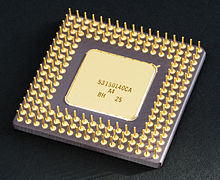
\includegraphics[scale=0.4]{Microprocesseur.jpg}
                \caption{Exemple de Microprocesseur}
                \label{fig: Exemple de Microprocesseur}
            \end{figure}

        \subsection{Fonctionnement}
            Un processeur n'est pas qu'une unité de calcul, il fait aussi appel à une unité de contrôle, une unité d'entrée-sortie,à une horloge et à des registres. \\
            Le séquenceur, ou unité de contrôle se charge de gérer le processeur. Il peut décoder les instructions, choisir les registres à utiliser, gérer les interruptions ou initialiser les registres au démarrage. Il fait appel à l'unité d'entrée-sortie pour communiquer avec la mémoire ou les périphériques. \\
            L'horloge doit fournir un signal régulier pour synchroniser tout le fonctionnement du processeur. Elle est présente dans les processeurs synchrone mais absente des processeurs asynchrones et des processeurs auto synchrones. \\
            Les registres sont des petites mémoires internes très rapides, pouvant être accédées facilement. Un plus grand nombre de registres permettra au processeur d'être plus indépendant de la mémoire. La taille des registres dépend de l'architecture, mais est généralement de quelques octets et correspond au nombre de bit de l'architecture (un processeur 8 bits aura des registres d'un octet). \\
            Il existe plusieurs registres, dont l'accumulateur et le compteur ordinal qui constituent la structure de base du processeur. Le premier sert à stocker les données traitées par l'UAL\footnotemark[2], et le second donne l'adresse mémoire de l'instruction en cours d'exécution ou de la suivante.
    
    \footnotetext[1]{central processing unit}
    \footnotetext[2]{unité de calcul arithmétique et logique}
    
    \newpage
    
    \section{Refroidisement}
    
        \subsection{Importance}
            Avoir un refroidissement efficace est aussi important que d'avoir un processeur ou une carte mere dans un ordinateur car sans cette piece capital les composants ce détruit bien plus vite voir n'arrive pas a démarer (systeme fail-safe\footnotemark[1])
            
        \subsection{Fonctionnement}
        
            \subsubsection{Refroidissement à air ou ventirad}
                \begin{itemize}
                    \item Refroidissement passif : Dans le cas d'un refroidissement passif, un simple dissipateur thermique (radiateur) est fixé sur l'élément à refroidir. Composé d'un métal à forte conductivité thermique comme le cuivre ou l'aluminium, La chaleur émise par le composant passe par le dissipateur thermique et est ensuite dissipée dans l'air ambiant.Afin d'assurer un contact, un transfert thermique efficace entre le composant et le dissipateur thermique, de la pâte thermique est souvent appliquée. \\
        
                    \item Refroidissement actif : Le refroidissement actif reprend le dissipateur thermique du refroidissement à air passif et lui adjoint des caloduc et un ventilateur afin d'être plus performant. Le bloc formé par le dissipateur, les caloducs et le ventilateur est souvent appelé ventirad (de ventilateur-radiateur).
                \end{itemize}
                
            \subsubsection{Refroidissement à eau ou Watercooling}
                Le watercooling est une technique destinée au refroidissement liquide des principaux composants d'un PC. Couramment, un ordinateur se refroidit par l'air par le biais d'un radiateur en aluminium qui capte la chaleur du composant (le processeur par exemple) et par un ventilateur dissipant la chaleur emmagasinée par le radiateur. \\
                En comparaison avec le ventirad, le refroidissement des composants par de l'eau est plus intéressant dans certains domaines. Tout d'abord, de par ses propriétés physiques de fluide caloporteur, l'eau conduit mieux la chaleur. Ensuite, l'eau est plus dense que l'air : pour refroidir une quantité de chaleur équivalente, il faut donc moins d'eau.
    
    \footnotetext[1]{systeme de sécurité}
    
    \newpage
    
    \section{Mémoire vive ou volatile (RAM)\protect\footnotemark[1]}
    
        \subsection{Fonctionnement}
            La mémoire vive est constituée de centaines de milliers de petits condensateurs emmagasinant des charges. Lorsqu'il est chargé, l'état logique du condensateur est égal à 1, dans le cas contraire il est à 0, ce qui signifie que chaque condensateur représente un bit de la mémoire.
            Etant donné que les condensateurs se déchargent, il faut constamment les recharger (le terme exact est rafraîchir) à un intervalle de temps régulier appelé cycle de rafraîchissement. Les mémoires RAM nécessitent par exemple des cycles de rafraîchissement est d'environ 15 nanosecondes (ns).\\
            Chaque condensateur est couplé à un transistor permettant de « récupérer » ou de modifier l'état du condensateur. Ces transistors sont rangés sous forme de tableau (matrice), c'est-à-dire que l'on accède à une case mémoire  par une ligne et une colonne.
            
        \subsection{Latence CAS\protect\footnotemark[2]}
            La latence CAS est toujours indiqué sur une barrette de RAM car cela indique la fréquence et la latence que va mettre la barrette pour inscrire les données a enregistré dans une rangée (RAS\footnotemark[3]).

        \begin{table}[h!]
        \begin{centering}
            \begin{tabular}{|C{3cm}|C{3cm}|C{3cm}|C{3cm}|C{3cm}|}
                \hline \rowcolor{gray} TECHNOLOGIE & VITESSE DU MODULE (MT/s) & DURÉE DU CYCLE D'HORLOGE (ns) & LATENCE CAS (CL) & VÉRITABLE LATENCE(ns) \\
                \hline \rowcolor{lightgray} DDR2 & 667 & 3.00 & 5 & 15.00 \\
                \hline  DDR2 & 800 & 2.50 & 6 & 15.00 \\
                \hline \rowcolor{lightgray} DDR3 & 1333 & 1.50 & 9 & 13.50 \\
                \hline  DDR3 & 1608 & 1.25 & 11 & 13.75 \\
                \hline \rowcolor{lightgray} DDR4 & 1866 & 1.07 & 13 & 13.93 \\
                \hline  DDR4 & 2133 & 0.94 & 15 & 14.06 \\
                \hline \rowcolor{lightgray} DDR4 & 2400 & 0.83 & 17 & 14.17 \\
                \hline  DDR4 & 2666 & 0.75 & 18 & 13.50 \\
                \hline
            \end{tabular}
            \caption{Tableau montrant la mesure de la véritable latence. \citep{site1}}
            \label{fig:Tableau montrant la mesure de la véritable latence.}
        \end{centering}
        \end{table}
    
    \footnotetext[1]{Random Access Memory}
    \footnotetext[2]{Column Address Strobe}
    \footnotetext[3]{Row Address Strobe}
    
    \newpage
    
    \section{Mémoire morte ou non volatile (ROM)\protect\footnotemark[1]}
        Elle permet de sauvegarder des données qui sont utile a l'utilisateur et a la machine. Contrairement a la mémoire vive qui enregistre les informations dans l'instantané mais qui une fois l'ordinateur éteins est vide car il n'y a plus d'alimentation.
        
        \subsection{Interne}
            le stockage interne comme indique sont nom est placé dans la machine dans des endroit normalement spécifiquement fait pour cela qui sont appeler des chambres de rangements pour éviter d’encombrer le flux d'air qui passe dans le boîtier d'un ordinateur par exemple.\\
            
            \begin{itemize}
                \item Disque dur (HDD)\footnotemark[2] :
                    Un ordinateur fonctionne de manière binaire ; il faut donc stocker les données sous forme de 0 et de 1. Avec un disque dur mécanique, les têtes de lecture-écriture sont dites « inductives » : elles sont capables de générer un champ magnétique positif ou négatif qui permet de polariser la surface du disque en une très petite zone.\\
                        \begin{figure}[h!]
                            \centering
                            \includegraphics[scale=0.07]{disque_dur.jpg}
                            \caption{Exemple de HDD}
                            \label{fig: Exemple de HDD}
                        \end{figure}
                \item SSD\footnotemark[3] :
                    C'est un matériel informatique permettant le stockage de données sur de la mémoire flash. La mémoire flash est une mémoire possédant les caractéristiques d'une mémoire vive mais dont les données ne disparaissent pas lors d'une mise hors tension. La mémoire flash stocke dans des cellules de mémoire les bits de données qui sont conservées lorsque l'alimentation électrique est coupée.
                    \begin{figure}[h!]
                        \centering
                        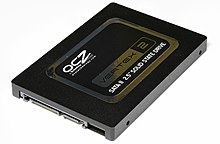
\includegraphics[scale=0.4]{SSD.jpg}
                        \caption{Exemple de SSD}
                        \label{fig: Exemple de SSD}
                    \end{figure}
            \end{itemize}
            
    \newpage
          
        \subsection{Externe}
        Il existe aussi des stockage externe appeler "périphérique de stockage" qui permette de transporter des données dans n'importe quel endroit de la planètes et de les connecter a différents appareils. \\
        
            \begin{itemize}
                \item Disque dur externe :
                    c'est le même fonctionnement que le hdd classique qui ce trouve dans une machine mais optimiser pour pouvoir être transporté qui a remplacer anciennement les disquettes \\
                    \begin{figure}[h!]
                        \centering
                        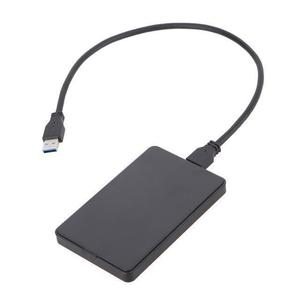
\includegraphics[scale=0.4]{Disque_dur_externe.jpg}
                        \caption{Exemple de Disque dur externe}
                        \label{fig: Exemple de Disque dur externe}
                    \end{figure}
                \item Clé usb : 
                    C'est un fonctionnement de stockage plus basique et le plus utiliser qui sert a stocké des données mais en plus petite quantité que le disque dur par exemple et très utile par sa taille et son poids.
                    \begin{figure}[h!]
                        \centering
                        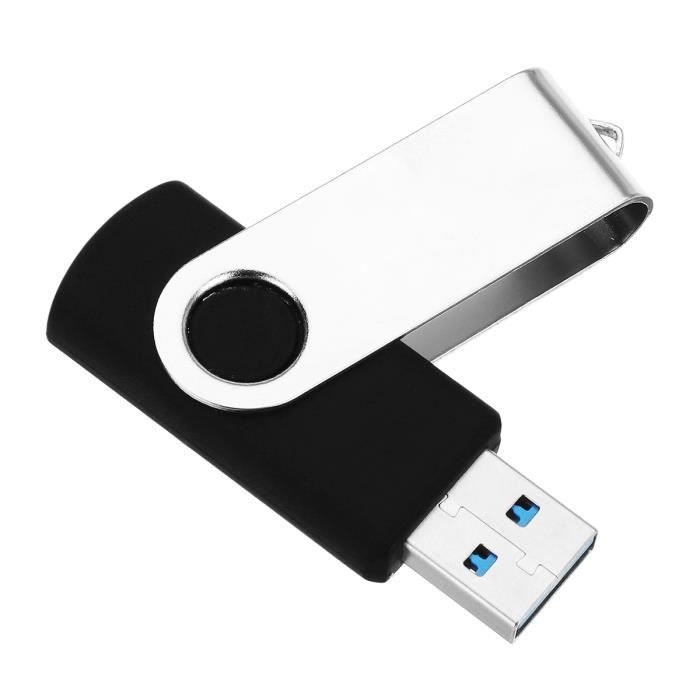
\includegraphics[scale=0.2]{Cle_USB.jpg}
                        \caption{Exemple de clé USB}
                        \label{fig: Exemple de clé USB}
                    \end{figure}
            \end{itemize}
            
    \footnotetext[1]{Read Only Memory}
    \footnotetext[2]{hard disk drive}
    \footnotetext[3]{solid-state drive}
    
    \newpage
    
    \section{Carte Mere}
        La carte mère est le circuit imprimé qui supporte la plupart des composants et des connecteurs nécessaires au fonctionnement d'un PC. \\
        Elle est essentiellement composée de circuits imprimés et de ports de connexion qui assurent la liaison de tous les composants et périphériques propres à un micro-ordinateur (disques durs (HDD/SSD), mémoire vive, microprocesseur, périphériques (souris, clavier, écran), etc.). \\
        Afin qu'ils puissent être reconnus et configurés par le microprocesseur grâce au programme contenu dans le BIOS\footnotemark[1] et qui faut souvent mettre a jour avec le site du fabricants de la carte mère pour mettre a jour aussi les pilotes contenus des périphérique et des composants de l'ordinateur.
        \begin{figure}[h!]
            \centering
            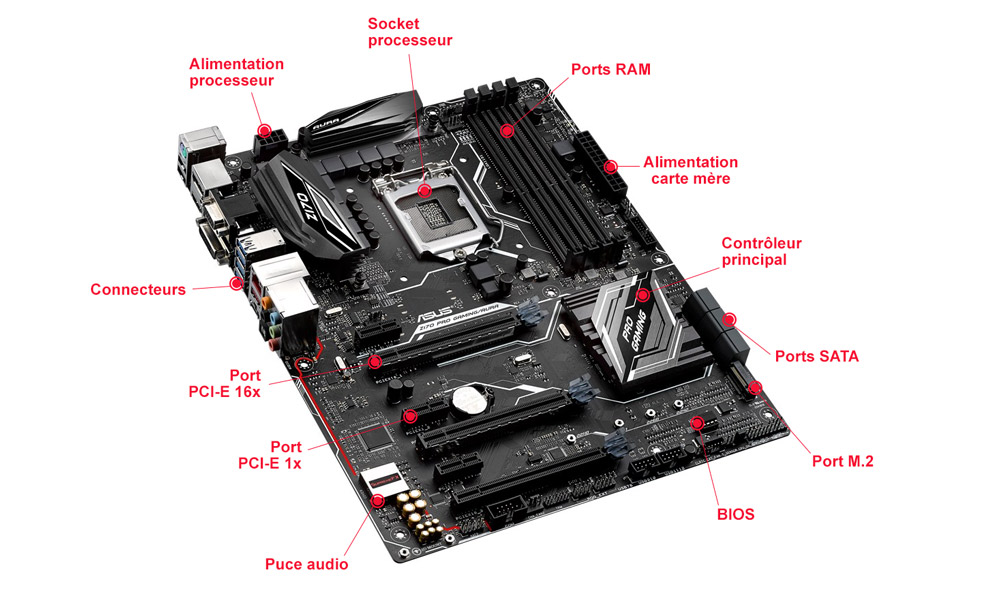
\includegraphics[scale=0.45]{Carte_mere.jpg}
            \caption{Exemple de Carte mère}
            \label{fig: Exemple de Carte mère}
        \end{figure}
   
   \footnotetext[1]{basic input output system} 
   
    \newpage
        
        \subsection{Fonctionnement}
            La carte mère sert a relier tout les composants d'un ordinateur entre eux pour pouvoir les utiliser convenablement et avec une certaine optimisation les socket qui sont mit en exemple ci-dessous montre les deux principaux fabricants de prosecteurs avec les références des socket qui sont utiliser pour insérer les processeur dans la carte mère. Cela donne l'information de la structure de la carte mère avec certain avantage de certaine technologique chez AMD comme chez INTEL. \\
            A Savoir : les carte mères ont plusieurs format qui sont ATX/mini-ATX/micro-ATX
            cela change juste la taille de tout les composants de la cartes mère qui peut donc accueillir moins ou plus de port PCI Exprès ou de barrettes de RAM.
    
            \subsubsection{socket}
                \begin{table}[h!]
                \begin{center}
                    \begin{tabular}{|C{2cm}||C{2.5cm}|C{3cm}||C{3cm}|C{4cm}|}
                        \hline \rowcolor{gray} ANNEE & REFERENCE & AMD & REFERENCE & INTEL \\
                        \hline \rowcolor{lightgray} 2004 & & & LGA 775 & Core 2, Pentium \\
                        \hline  2006 & AM2 & Athlon 64 & & \\
                        \hline \rowcolor{lightgray} 2007 & AM2+ & Phenom, Atlhon 64 & P & Core 2  \\
                        \hline  2008 & AM3 & Phenom II, Atlhon II & LGA 771 & Xeon, Intel core 2 \\
                        \hline \rowcolor{lightgray} 2009 & ASB1 & Athlon neo, turion neo & LGA 1156 & Core I5, Core I7  \\
                        \hline  2011 & & & LGA 1155 & Pentium I3, I5, I7 \\
                        \hline \rowcolor{lightgray} 2013 & & & LGA 1150 & Pentium I3, I5, I7  \\
                        \hline  2015 & & & LGA 1151 & Pentium I3, I5, I7 \\
                        \hline \rowcolor{lightgray} 2017 & AM4, TR4 & Ryzen, Threadtripper & LGA 2066 & I5, I7, I9 \\
                        \hline  2020 & & & LGA 1200 & Celeron, I3, I5, I7, I9 \\
                        \hline
                    \end{tabular}
                    \caption{Tableau montrant les différents socket par années et constructeurs. \citep{site2}}
                    \label{fig:Tableau montrant les différents socket par années et constructeurs.}
                \end{center}
                \end{table}
    
    \newpage
    
    \bibliographystyle{plain}
    \bibliography{references}
\end{document}